\documentclass[12pt]{report}
\usepackage{graphicx}
\usepackage[utf8]{inputenc}
\usepackage[spanish]{babel}
\usepackage{setspace}
\usepackage{geometry}
\usepackage{titlesec}
\usepackage{times}
\usepackage{mathptmx} % Use mathptmx instead of times
\usepackage{fancyhdr}
\usepackage{hyperref}
\usepackage{float}


% Configuración de márgenes
\geometry{
    top=2.5cm,
    left=3cm,
    right=3cm,
    bottom=2.5cm
}

% Configuración de interlineado
\onehalfspacing

% Configuración de títulos y subtítulos
\titleformat{\chapter}[display]
  {\normalfont\bfseries\centering}{}{0pt}{\fontsize{14}{16}\selectfont}
\titleformat{\section}
  {\normalfont\bfseries}{\thesection}{1em}{\fontsize{12}{14}\selectfont}
\titleformat{\subsection}
  {\normalfont\bfseries}{\thesubsection}{1em}{\fontsize{12}{14}\selectfont}


% Configuración de pie de página
  \fancyhf{}
\fancyfoot[R]{\thepage}
\pagestyle{fancy}
\fancypagestyle{plain}{
  \fancyhf{}
  \fancyfoot[R]{\thepage}
}

  \begin{document}
  \pagenumbering{roman}
%----- PORTADA ----
\setlength{\hoffset}{27 pt} % 1 (Para centrar más la portada)
\begin{titlepage}
{\centering
{\fontfamily{ptm}\scshape\bfseries\fontsize{29.16}{34.992}\selectfont Universidad de Guadalajara \par}
\vspace{0.5cm}
{\scshape\Large Centro Universitario de los Lagos \par}
\vspace{1cm}
{\scshape\Large División de Estudios de la Biodiversidad e innovación Tecnológica \par}
\vspace{1cm}
{\graphicspath{{imagenes/Portada}} %ruta de las imagenes

\includegraphics[width=0.3\textwidth]{image.png}\par}
\vspace{1cm}
% Título
{\scshape\large\bfseries Esquematico \par}
\vspace{1.5cm}
% Materia
{\large \textbf{Asignatura:} \\Diseño Electronico Asistido por Computadora\par}
\vfill
% Estudiante
{\large \textbf{Presenta:} \\Oscar Iván Moreno Gutiérrez \#220942754\par}
\vfill
% Profesor
{\large \textbf{Profesor:} \\Mtro. Jaime Eduardo Pons Arenas \par}
\vfill
\vfill
% Fecha
\begin{flushright}
  {\normalsize \textbf {Fecha:} \\ \today}
\end{flushright}
\vfill}
{\large  \par}
\end{titlepage}
%----- FIN DE PORTADA ----

%----- ÍNDICE GENERAL ----
\tableofcontents
\newpage



%----- OBJETIVO ----
\chapter*{Objetivo}
\addcontentsline{toc}{chapter}{Objetivo}
El objetivo de esta actividad es hacer el esquematico del proyecto del colorimetro.
\newpage

%----- CONTENIDO ----
\chapter{Contenido}
\section{Utilizacion de Fusion 360}
  Se utilizo el programa de diseño 3D Fusion 360 para realizar el diseño del colorimetro.
Razones por las que se eligio Fusion 360:
\begin{itemize}
  \item Facilidad de uso: Fusion 360 es un programa muy intuitivo y fácil de usar.
  \item Herramientas de diseño: Fusion 360 cuenta con una gran cantidad de herramientas de diseño que permiten crear modelos 3D de alta calidad, ademas de una libreria amplia de componentes electronicos cons sus respectivos footprints.
\end{itemize}



\section{En que nos basamos para el diseño?}
  Nos basamos en el diseño de un colorímetro que se encuentra en la página de Instructables: \href{https://www.instructables.com/Your-Own-Color-Sensor-using-LEDs/}{Your Own Color Sensor using LEDs}.

  Que se modifico para conecta a un microcontrolador MSP430
  %% Imagen aqui
  \begin{figure}[H]
    \centering
    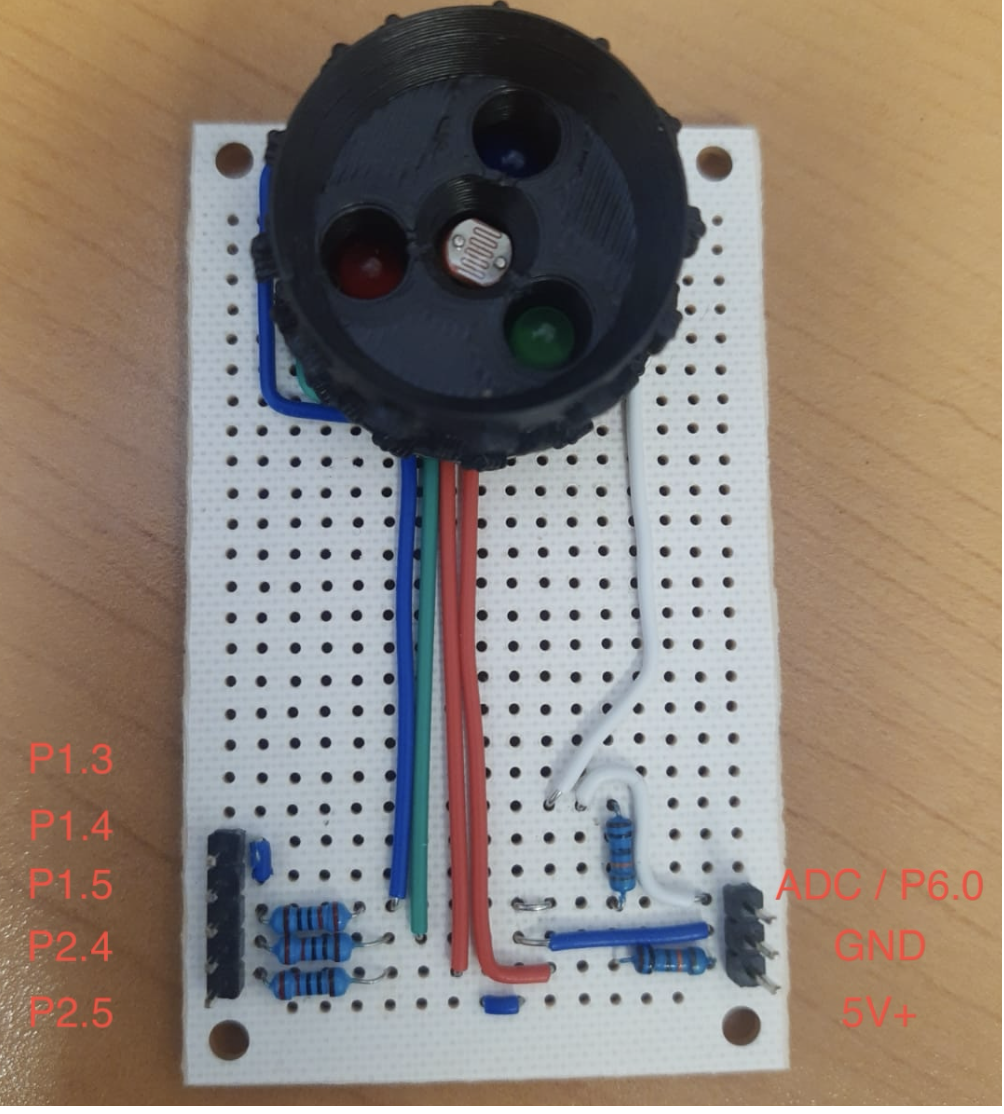
\includegraphics[width=0.5\textwidth]{circuito_MSP.png}
    \caption{Colorimetro}
    \label{fig:colorimetro}
  \end{figure}
  Se puede observar que tenemos 8 pines en el circuito, los cuales se conectan a los pines del MSP430:
  \begin{itemize}
    \item Pin 1.3: se conecta con el puerto 1.3 y se puentea con el 1.4
    \item Pin 1.4: se conecta con el puerto 1.4 y se puentea con el 1.3
    \item Pin 1.5: se controla para el led Azul
    \item Pin 2.4: se controla para el led Verde
    \item Pin 2.5: se controla para el led Rojo
    \item Pin 6.0: se conecta al ADC
    \item Pin GND: GND
    \item Pin VCC: 5V+
  \end{itemize}
Se monta de la siguiente manera:
\begin{figure}[H]
  \centering
  \includegraphics[width=0.5\textwidth]{uso_adecuado.png}
  \caption{Uso adecuado}
  \label{fig:uso_adecuado}
\end{figure}

\section{Componentes}
\begin{figure}[H]
  \centering
  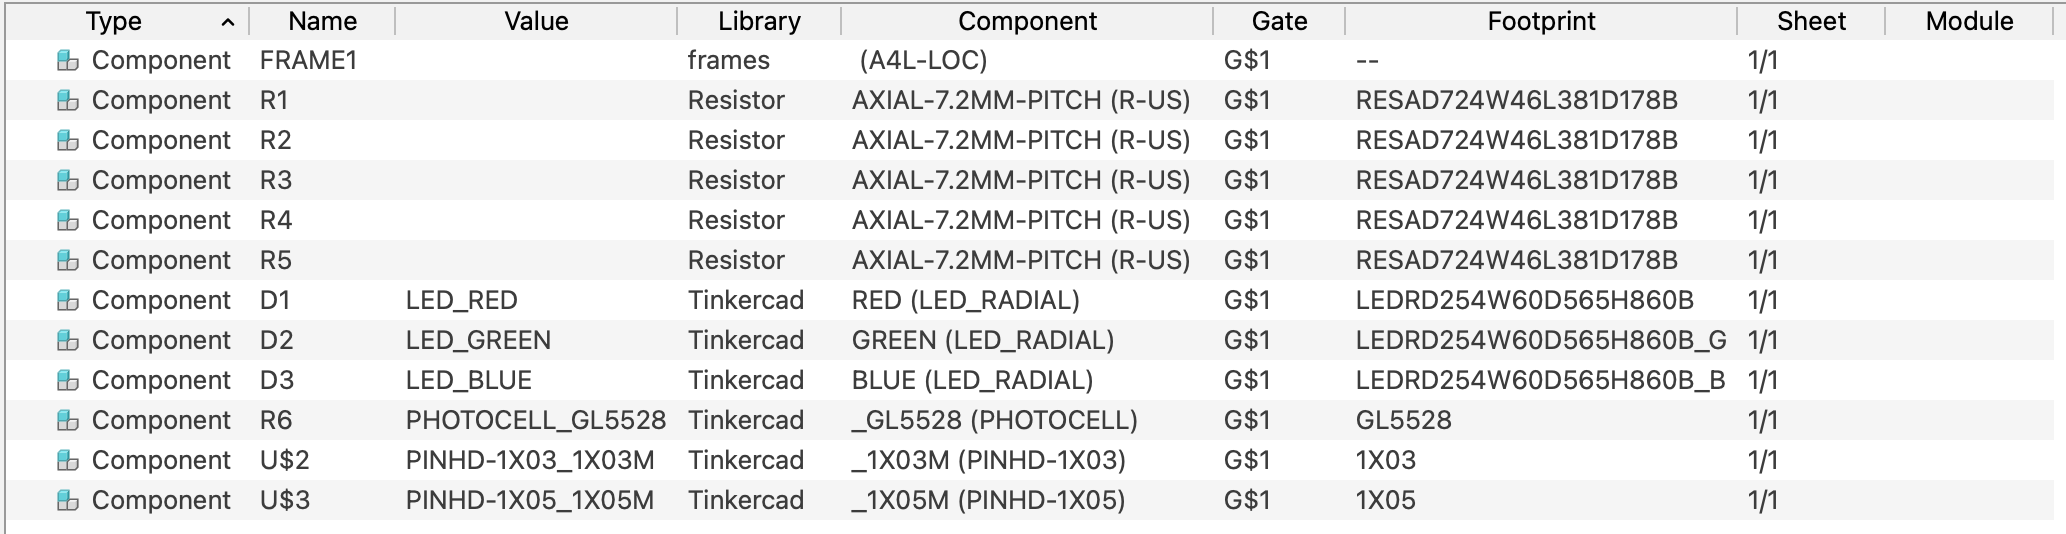
\includegraphics[width=1.0\textwidth]{Componentes.png}
  \caption{Componentes}
  \label{fig:Componentes} 
\end{figure}
\section{Circuito}
Ya que tenemos los componentes, procedemos a armar el circuito.
\begin{figure}[H]
  \centering
  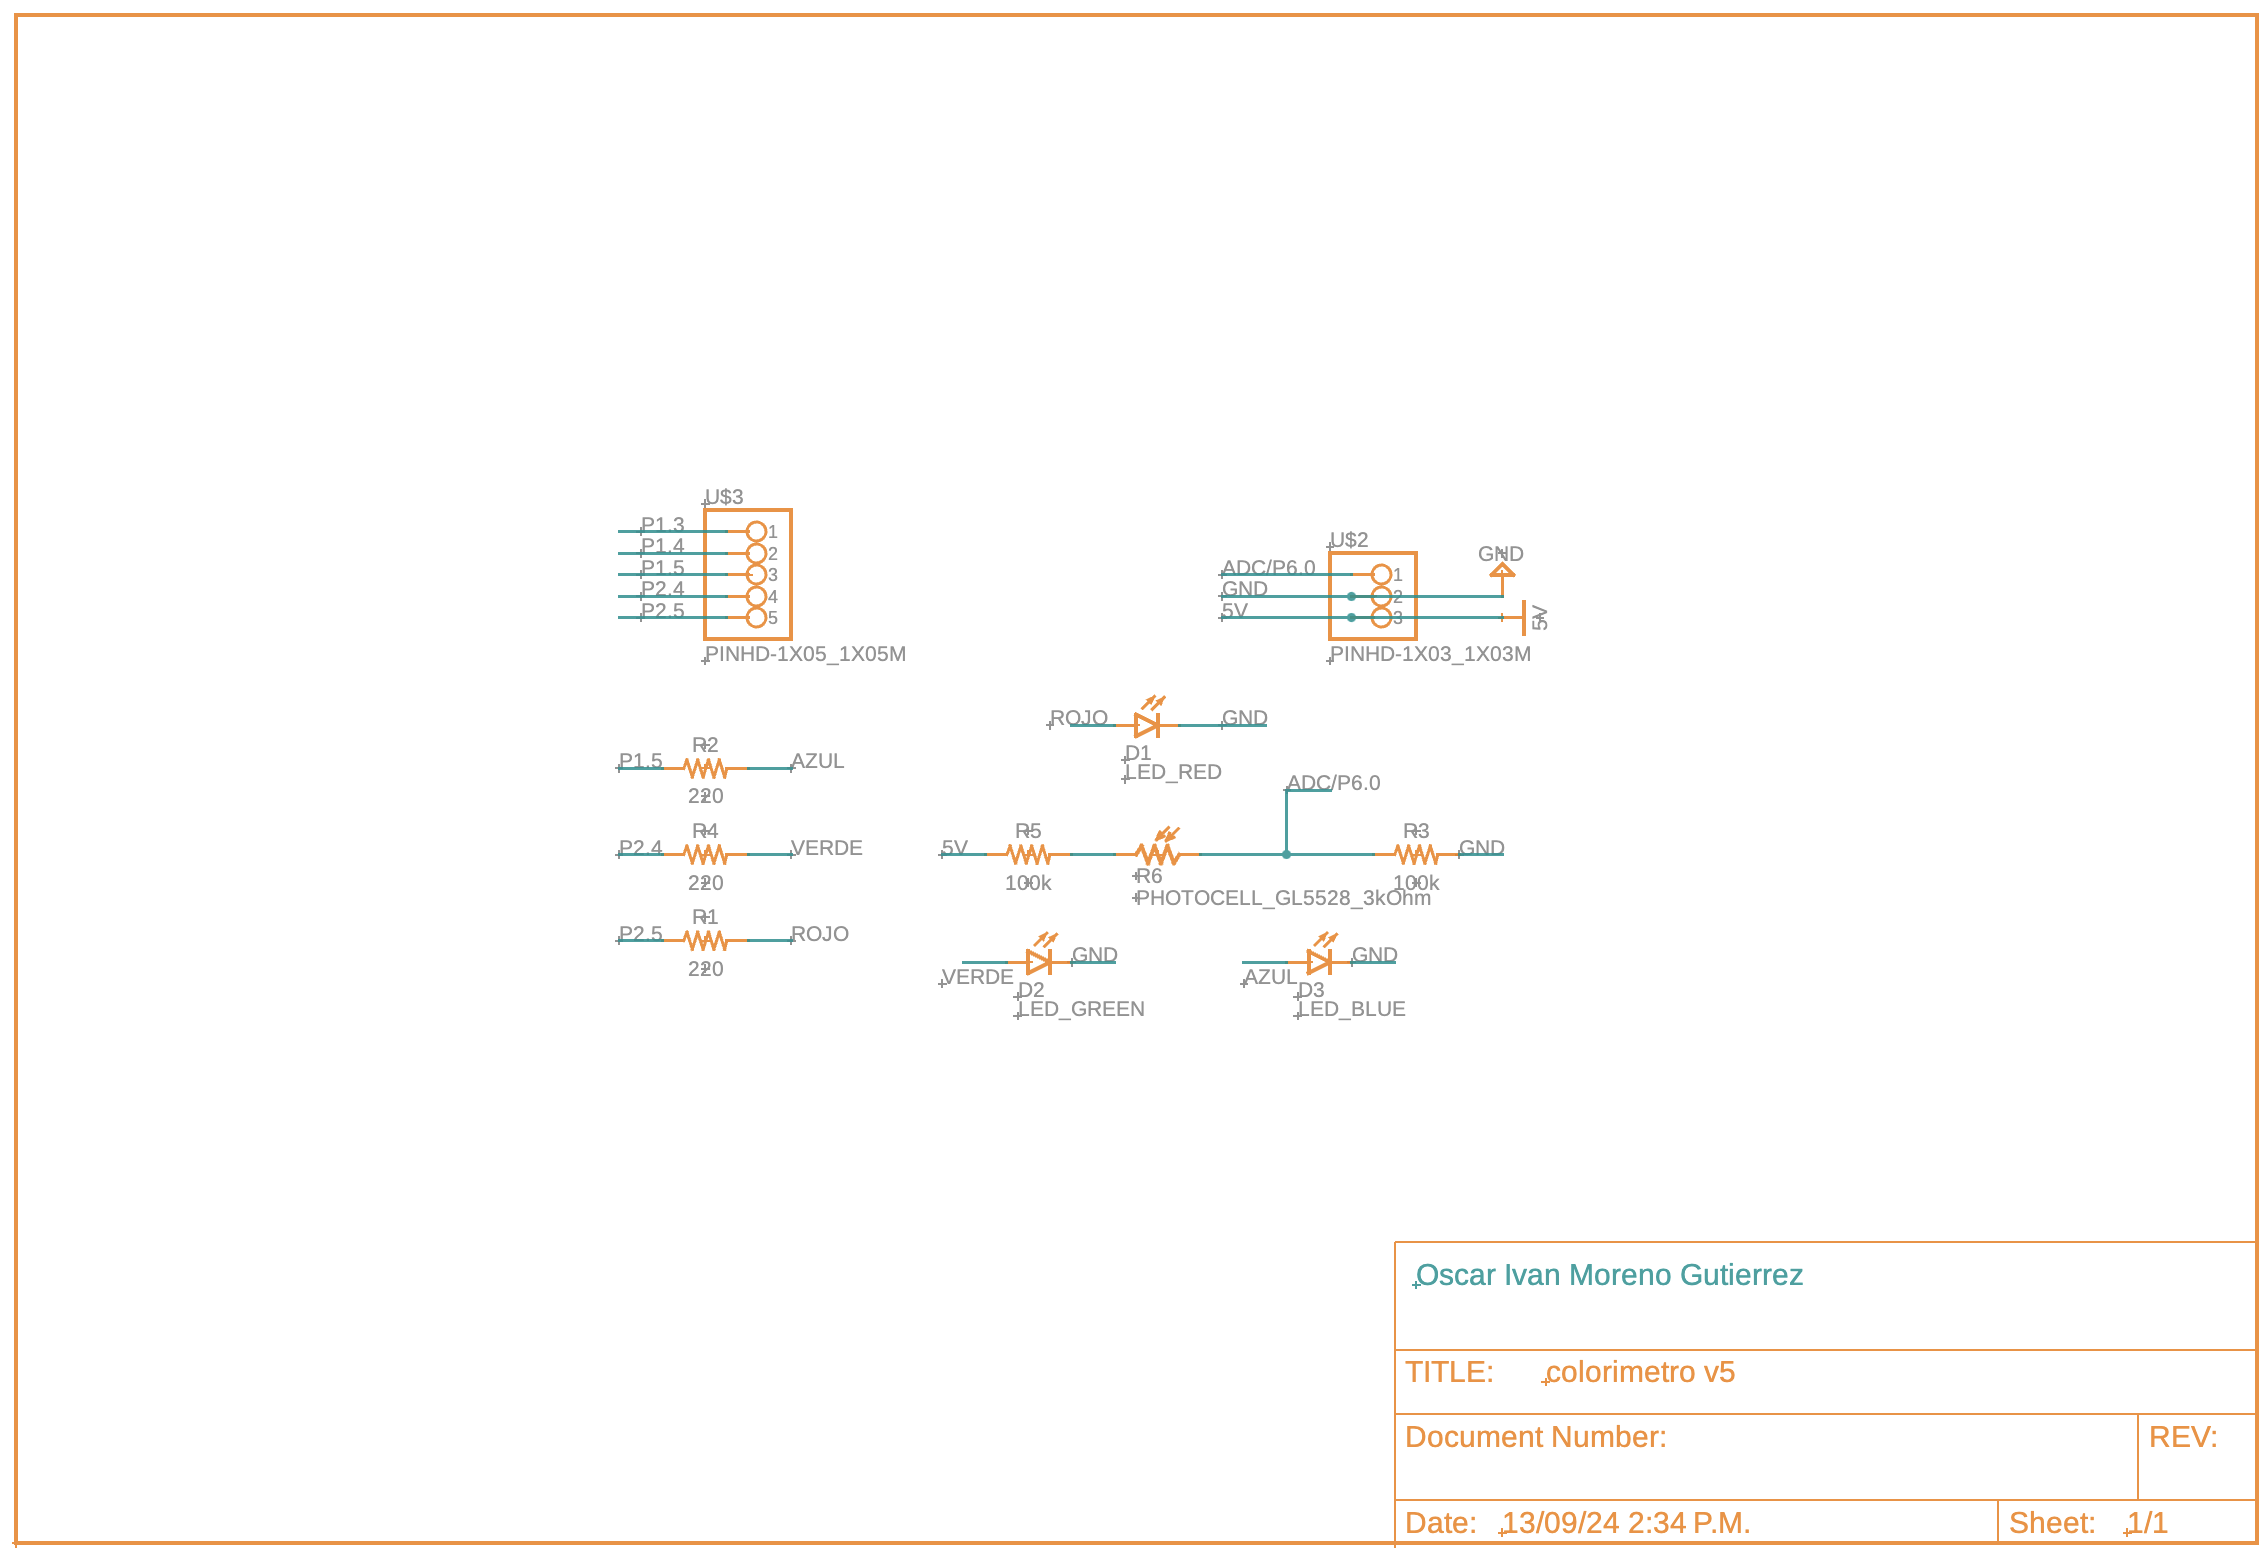
\includegraphics[width=1.5\textwidth, angle=90]{esquematico.png}
  \caption{Circuito}
  \label{fig:Circuito}
\end{figure}
\newpage
\end{document}